\chapter{Compare element 8-nodes element 4-nodes in solving the contact examples} % Main chapter title

\label{Chapter5 } % For referencing the chapter elsewhere, use \ref{Chapter1} 
In this chapter, we re-solve two examples (self-contact example and rubber blade example) using 8-nodes and 4-nodes elements. The results calculated by the MATLAB program are compared with the results of the ANSYS software corresponding to the 8-nodes and 4-nodes elements (that is, the MATLAB calculation results of the 8-nodes element will be compared with the simulation results above. ANSYS software of the 8-nodes element, similarly for the 4-nodes element).
\vspace{0.38cm}
\newline
It makes no sense for us to compare 8-nodes element and 4-nodes element on the same element size. Thus, of course, using the 8-nodes element will give more accurate results. In this chapter, when using an element of 8-nodes, the size of the element will be four times larger than the size of a 4-nodes element (represented in the Figure \ref{fig:dif4-nodes8-nodes}).
\vspace{0.38cm}
\newline
Maximum volume displacement and maximum stress are compared in this chapter.
\newline
\begin{figure}[H]
    \centering
    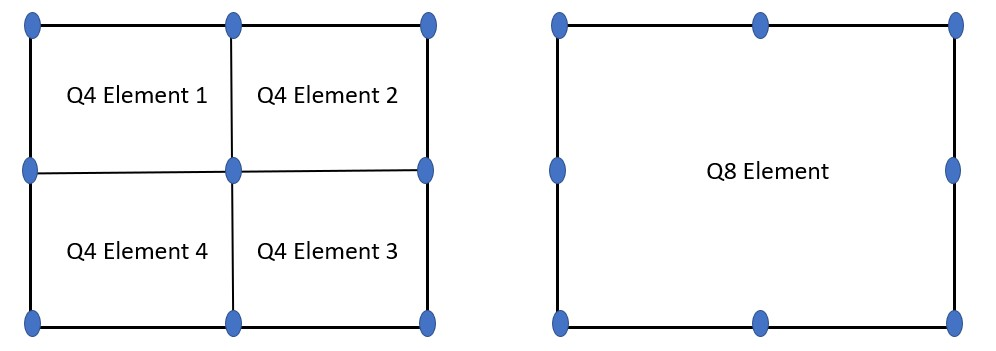
\includegraphics[scale=0.5]{Figures/chapter5/difQ4Q8.jpg}
    \decoRule
    \caption{Differences in meshing}
    \label{fig:dif4-nodes8-nodes}
\end{figure}
\newpage
\section{Self-contact example}
With the model and boundary conditions as in the previous chapter, we solve the problem using 8-nodes and 4-nodes elements.
\subsection{Mesh and solution time}
Material props: Neo-hookean model with material properties: the shear modulus ($\mu$) is assumed to be $80.194 N/mm^2$ and the bulk modulus ($\kappa$) is $120.291 N/mm^2$.
\vspace{0.38cm} \newline
Frictionless: in this study, contact problems with hyper-elastic materials are
considered in cases of frictionless sliding and frictionless compressing.
\vspace{0.38cm} \newline
Boundary conditions: in this example, we have the following boundary conditions: the Bottom edge is 
constrained displacement in the two directions x, y; Top edge is constrained to displacement in the 
x direction and is applied displacement is $u_y = - 6 mm$.
\vspace{0.38cm}
\newline
The case of meshing with 8-nodes is shown in Figure \ref{fig:q8_mesh_s}.
While for meshing with a 4-nodes element, it is shown in Figure \ref{fig:q4_mesh_s}.
Table \ref{tab:mp_s} shows the total number of nodes and the total number of elements of the model when meshing by two element types.
\vspace{0.01cm}
\newline

\begin{figure}[H]
    \centering
    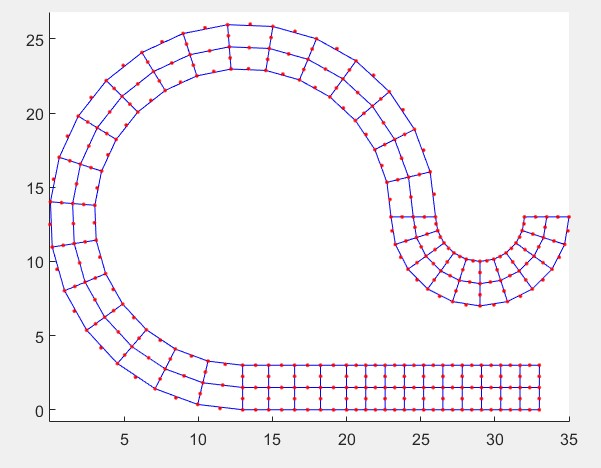
\includegraphics[scale=0.72]{Figures/chapter5/q8_mesh_s.jpg}
    \decoRule
    \caption{Mesh when using the 8-nodes element of self-contact example }
    \label{fig:q8_mesh_s}
\end{figure}

\begin{figure}[H]
    \centering
    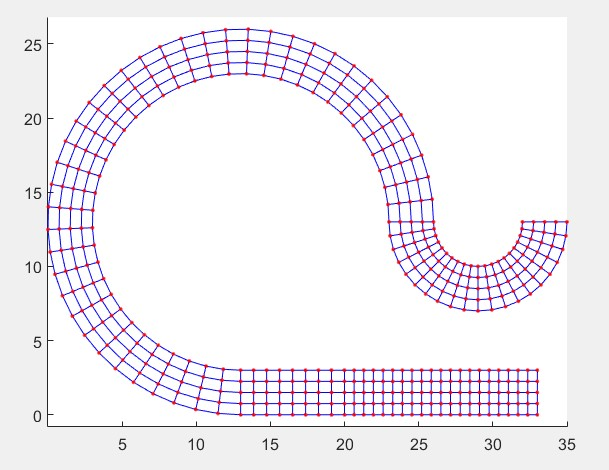
\includegraphics[scale=0.7]{Figures/chapter5/q4_mesh_s.jpg}
    \decoRule
    \caption{Mesh when using the 4-nodes element of self-contact example}
    \label{fig:q4_mesh_s}
\end{figure}
\begin{table}[H]
    \centering
    \scalebox{1}{
    \begin{tabular}{|c|c|c|}
    \multicolumn{3}{c}{Mesh properties} \\ \hline
         Element type & Total of node & Total of element \\ \hline 
         8-nodes      & 357        & 88 \\ \hline
         4-nodes      & 445        & 352 \\ \hline
    \end{tabular}}
    \caption{Mesh properties of self-contact example}
    \label{tab:mp_s}
\end{table}
\noindent
Although less in number of nodes and significantly less (four times) in number of elements, the solving time when using 8-nodes element is not much less than when using 4-nodes element.
The solving time is shown in the Table \ref{tab:st_s}
\begin{table}[H]
    \centering
    \begin{tabular}{|c|c|}
    \multicolumn{2}{c}{The solving time} \\ \hline
         Element type & Time \\ \hline 
         8-nodes           & 108s \\ \hline
         4-nodes           & 114s \\ \hline
    \end{tabular}
    \caption{The solving time of self-contact example}
    \label{tab:st_s}
\end{table}
\newpage
\subsection{Compare displacement}
%% COMPARE ux

% ux of q8
\begin{figure}[H]
    \centering
    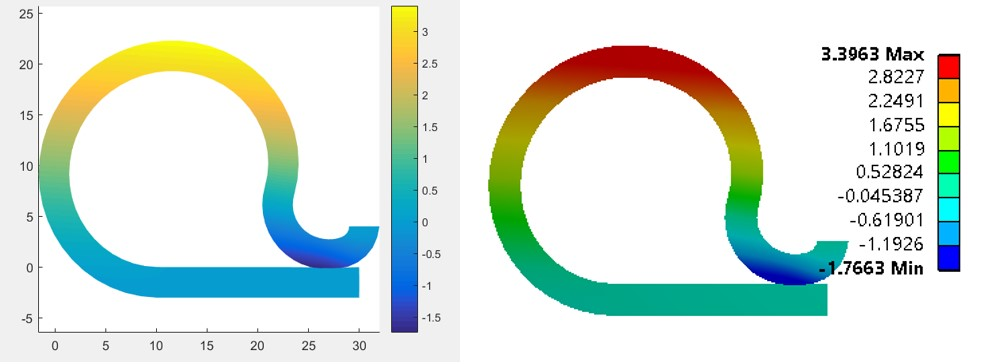
\includegraphics[scale=0.6]{Figures/chapter5/s_q8_ux.jpg}
    \decoRule
    \caption{$u_x$ displacement when using Q8 of self-contact example \\
    (MATLAB result in the left, ANSYS result in the right)}
    \label{fig:s_q8_ux}
\end{figure}
The $u_x$ displacement of self-contact example when using 8-nodes element is shown in the Figure \ref{fig:s_q8_ux}.
Maximum volume $u_x$ displacement of MATLAB result is $3.3923 mm$.
Maximum volume $u_x$ displacement of ANSYS result is $3.3963 mm$.
The error of maximum volume $u_x$ displacement between MATLAB result and ANSYS result when using 8-nodes element is $0.12\%$.
\newline

% ux of q4
\begin{figure}[H]
    \centering
    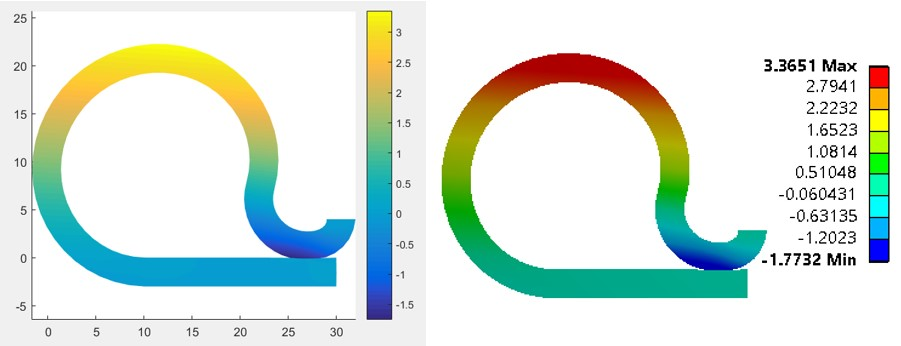
\includegraphics[scale=0.65]{Figures/chapter5/s_q4_ux.jpg}
    \decoRule
    \caption{$u_x$ displacement when using Q4 of self-contact example \\
    (MATLAB result in the left, ANSYS result in the right)}
    \label{fig:s_q4_ux}
\end{figure}
\noindent
The $u_x$ displacement of self-contact example when using 4-nodes element is shown in the Figure \ref{fig:s_q4_ux}.
Maximum volume $u_x$ displacement of MATLAB result is $3.3404 mm$.
Maximum volume $u_x$ displacement of ANSYS result is $3.3651 mm$.
The error of maximum volume $u_x$ displacement between MATLAB result and ANSYS result when using 4-nodes element is $0.73\%$.
So, for maximum volume $u_x$ displacement, the error when using 8-nodes element is lower than when using 4-nodes element.
\newpage
%% COMPARE uy
% uy of q8
\begin{figure}[H]
    \centering
    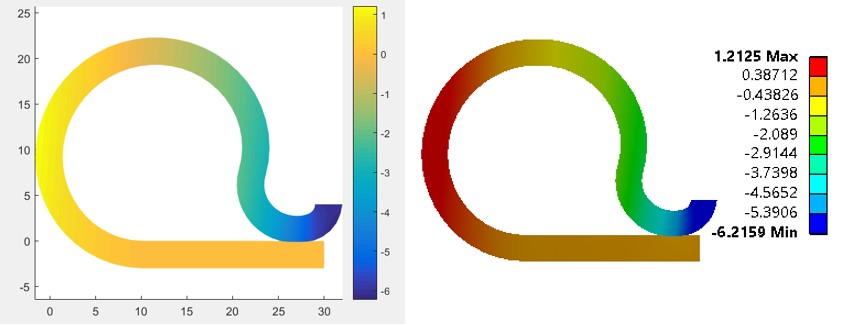
\includegraphics[scale=0.7]{Figures/chapter5/s_q8_uy.jpg}
    \decoRule
    \caption{$u_y$ displacement when using Q8 of self-contact example \\
    (MATLAB result in the left, ANSYS result in the right)}
    \label{fig:s_q8_uy}
\end{figure}
\noindent
The $u_y$ displacement of self-contact example when using 8-nodes element is shown in the Figure \ref{fig:s_q8_uy}.
Maximum volume $u_y$ displacement of MATLAB result is $6.2109mm$.
Maximum volume $u_y$ displacement of ANSYS result is $6.2159mm$.
The error of maximum volume $u_y$ displacement between MATLAB result and ANSYS result when using 8-nodes element is $0.08\%$.
\newline
% uy of q4
\begin{figure}[H]
    \centering
    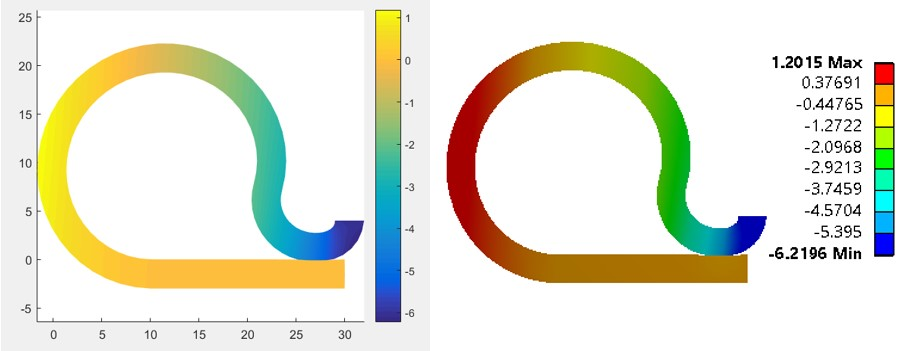
\includegraphics[scale=0.66]{Figures/chapter5/s_q4_uy.jpg}
    \decoRule
    \caption{$u_y$ displacement when using Q4 of self-contact example \\
    (MATLAB result in the left, ANSYS result in the right)}
    \label{fig:s_q4_uy}
\end{figure}
\noindent
The $u_y$ displacement of self-contact example when using 8-nodes element is shown in the Figure \ref{fig:s_q4_uy}.
Maximum volume $u_y$ displacement of MATLAB result is $6.2132mm$.
Maximum volume $u_y$ displacement of ANSYS result is $6.2196mm$.
The error of maximum volume $u_y$ displacement between MATLAB result and ANSYS result when using 8-nodes element is $0.1\%$.
So, for maximum volume $u_y$ displacement, the error when using 8-nodes element is lower than when using 4-nodes element.
\vspace{0.38cm}
\newline
Thus, for the self-contact example, using the 8-nodes element gives more accurate displacement results than using the 4-nodes element.
\newpage
\subsection{Compare stress distribution}
%% COMPARE SX
% sx of q8
\begin{figure}[H]
    \centering
    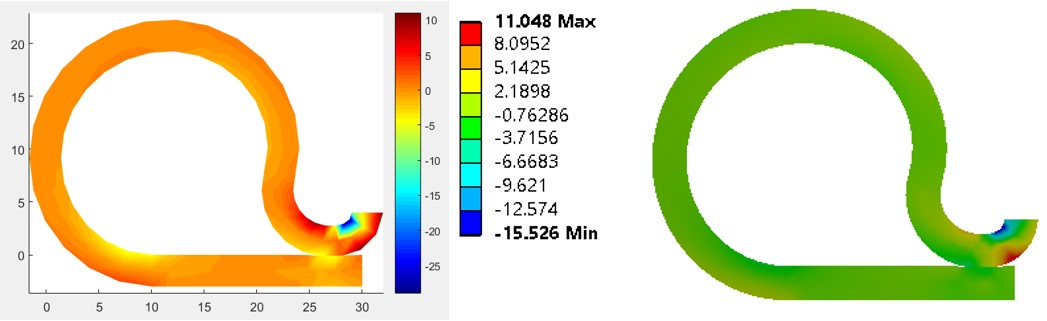
\includegraphics[scale=0.575]{Figures/sx_self_MandA.jpg}
    \decoRule
    \caption{Normal stress $\sigma_x$ when using Q8 of self-contact example \\
    (MATLAB result in the left, ANSYS result in the right)}
    \label{fig:sx_self_MandA_5}
\end{figure}
\noindent
The normal stress $\sigma_x$ of self-contact example when using 8-nodes element is shown in the Figure \ref{fig:sx_self_MandA_5}.
Maximum normal stress $\sigma_x$ of MATLAB result is $10.9231 MPa$.
Maximum normal stress $\sigma_x$ of ANSYS result is $11.048 MPa$.
The error of maximum normal stress $\sigma_x$ between MATLAB result and ANSYS result when using 8-nodes element is $1.13\%$.
\newline
% sx of q4
\begin{figure}[H]
    \centering
    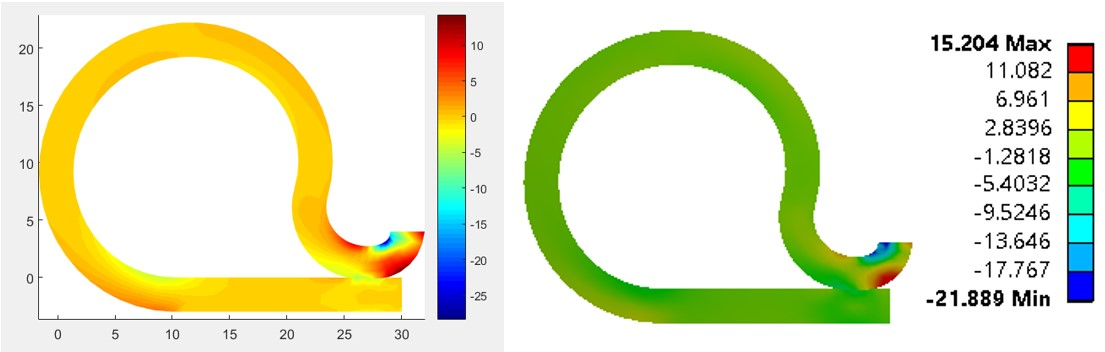
\includegraphics[scale=0.54]{Figures/chapter5/sx_q4_c.jpg}
    \decoRule
    \caption{Normal stress $\sigma_x$ when using Q4 of self-contact example \\
    (MATLAB result in the left, ANSYS result in the right)}
    \label{fig:sx_q4_c}
\end{figure}
\noindent
The normal stress $\sigma_x$ of self-contact example when using 4-nodes element is shown in the Figure \ref{fig:sx_q4_c}.
Maximum normal stress $\sigma_x$ of MATLAB result is $14.1402 MPa$.
Maximum normal stress $\sigma_x$ of ANSYS result is $15.204 MPa$.
The error of maximum normal stress $\sigma_x$ between MATLAB result and ANSYS result when using 8-nodes element is $7\%$.
So, for maximum normal stress $\sigma_x$, the error when using 8-nodes element is lower than when using 4-nodes element.
\newpage

%% COMPARE SY
% sx of q8
\begin{figure}[H]
    \centering
    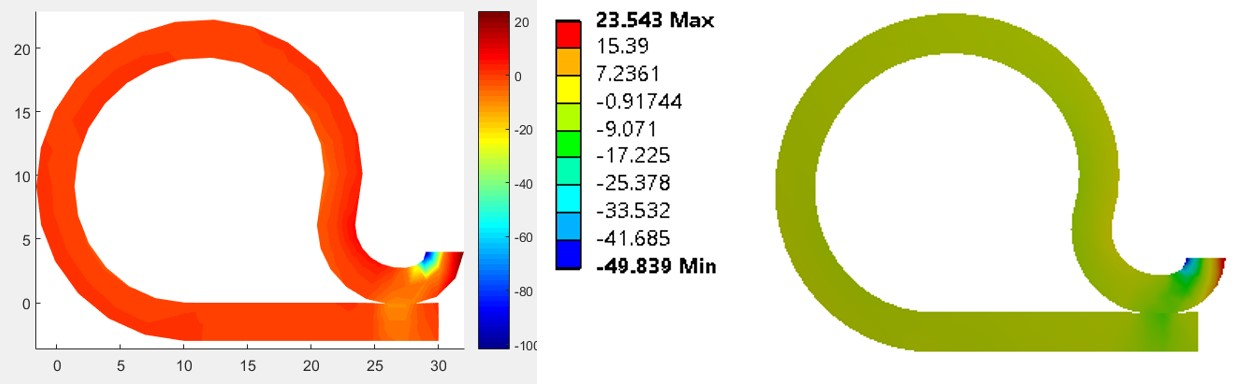
\includegraphics[scale=0.5]{Figures/sy_self_MandA.jpg}
    \decoRule
    \caption{Normal stress $\sigma_y$ when using Q8 of self-contact example \\
    (MATLAB result in the left, ANSYS result in the right)}
    \label{fig:sy_self_MandA_5}
\end{figure}
\noindent
The normal stress $\sigma_y$ of self-contact example when using 8-nodes element is shown in the Figure \ref{fig:sy_self_MandA_5}.
Maximum normal stress $\sigma_y$ of MATLAB result is $23.5783 MPa$.
Maximum normal stress $\sigma_y$ of ANSYS result is $23.543 MPa$.
The error of maximum normal stress $\sigma_y$ between MATLAB result and ANSYS result when using 8-nodes element is $0.18\%$.

% sx of q4
\begin{figure}[H]
    \centering
    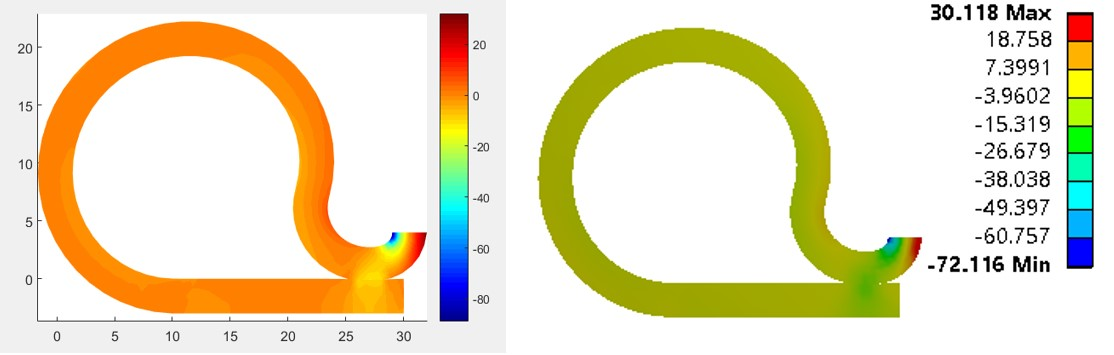
\includegraphics[scale=0.55]{Figures/chapter5/sy_q4_c.jpg}
    \decoRule
    \caption{Normal stress $\sigma_y$ when using Q4 of self-contact example \\
    (MATLAB result in the left, ANSYS result in the right)}
    \label{fig:sy_q4_c}
\end{figure}
\noindent
The normal stress $\sigma_y$ of self-contact example when using 4-nodes element is shown in the Figure \ref{fig:sy_q4_c}.
Maximum normal stress $\sigma_y$ of MATLAB result is $31.8452 MPa$.
Maximum normal stress $\sigma_y$ of ANSYS result is $30.118 MPa$.
The error of maximum normal stress $\sigma_y$ between MATLAB result and ANSYS result when using 8-nodes element is $5.7\%$.
So, for maximum normal stress $\sigma_y$, the error when using 8-nodes element is lower than when using 4-nodes element.
\vspace{0.38cm}
\newline
Thus, for the self-contact example, using the 8-nodes element gives more accurate normal stress results than using the 4-nodes element.
%%%%%%%%%%%%%%%%%%%%%%%%%%%%%%%%%%%%%%%%%%%%%%%%%%%%%%%%%%%%%%%%%%%%%%%%%%%%%%%%%%%%
\newpage
\section{Rubber blade example}
With the model and boundary conditions as in the previous chapter, we solve the problem using 8-nodes and 4-nodes elements.
\subsection{Mesh and solution time}
Material props: Neo-hookean model with material properties: the shear modulus ($\mu$) is assumed to be $80.194 N/mm^2$ and the bulk modulus ($\kappa$) is $60.291 N/mm^2$.
\vspace{0.38cm} \newline
Frictionless: in this study, contact problems with hyper-elastic materials are
considered in cases of frictionless sliding and frictionless compressing.
\vspace{0.38cm} \newline
Boundary conditions: in this example, we have the following boundary conditions: the Bottom edge is 
constrained displacement in the two directions x, y; Top edge is constrained to displacement in the 
x direction and is applied displacement is $u_y = - 2 mm$.
\vspace{0.38cm}
\newline
The case of meshing with 8-nodes is shown in Figure \ref{fig:q8_mesh_r}.
While for meshing with a 4-nodes element, it is shown in Figure \ref{fig:q4_mesh_r}.
Table \ref{tab:mp_r} shows the total number of nodes and the total number of elements of the model when meshing by two element types.
\vspace{0.01cm}
\newline
% mesh q8
\begin{figure}[H]
    \centering
    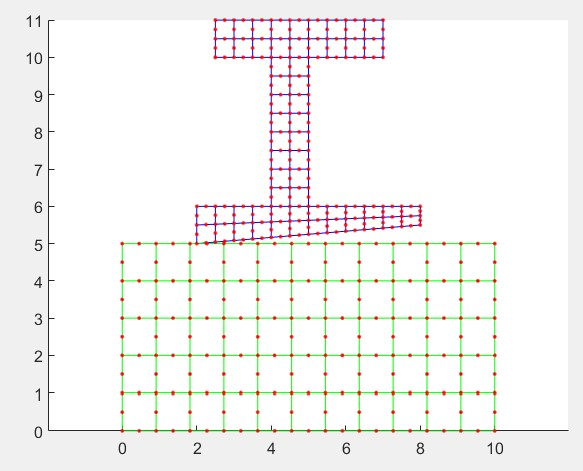
\includegraphics[scale=0.875]{Figures/chapter5/q8_mesh_r.jpg}
    \decoRule
    \caption{Mesh when using the 8-nodes element of rubber blade example}
    \label{fig:q8_mesh_r}
\end{figure}
%mesh q4
\begin{figure}[H]
    \centering
    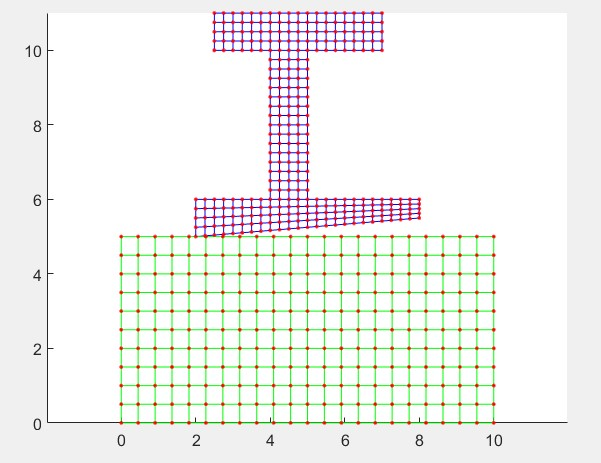
\includegraphics[scale=0.85]{Figures/chapter5/q4_mesh_r.jpg}
    \decoRule
    \caption{Mesh when using the 4-nodes element of rubber blade example}
    \label{fig:q4_mesh_r}
\end{figure}

\begin{table}[H]
    \centering
    \scalebox{1}{
    \begin{tabular}{|c|c|c|}
    \multicolumn{3}{c}{Mesh properties} \\ \hline
         Element type & Total of node & Total of element \\ \hline 
         8-nodes      & 435        & 113 \\ \hline
         4-nodes      & 548        & 452 \\ \hline
    \end{tabular}}
    \caption{Mesh properties of rubber blade example}
    \label{tab:mp_r}
\end{table}
\noindent
The solving time is shown in the Table \ref{tab:st_r}.
Although less in number of nodes and significantly less (four times) in number of elements, the solving time when using 8-nodes element is not much less than when using 4-nodes element.
\begin{table}[H]
    \centering
    \begin{tabular}{|c|c|}
    \multicolumn{2}{c}{The solving time} \\ \hline
         Element type & Time \\ \hline 
         8-nodes           & 75s \\ \hline
         4-nodes           & 79s \\ \hline
    \end{tabular}
    \caption{The solving time of self-contact example}
    \label{tab:st_r}
\end{table}
\newpage
\subsection{Compare displacement}
%% COMPARE ux

% ux of q8
\begin{figure}[H]
    \centering
    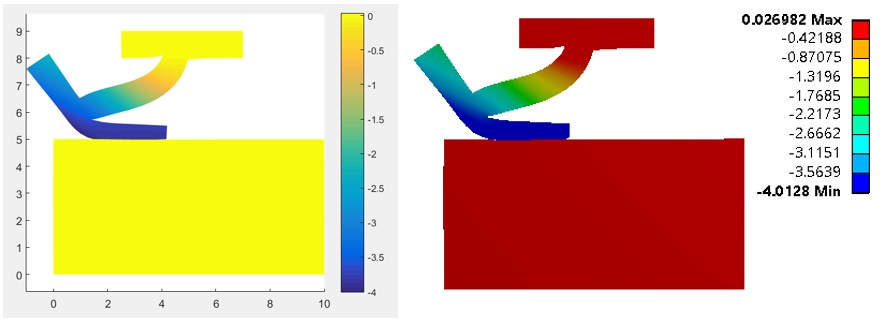
\includegraphics[scale=0.7]{Figures/chapter5/r_q8_ux.jpg}
    \decoRule
    \caption{$u_x$ displacement when using Q8 of rubber example \\
    (MATLAB result in the left, ANSYS result in the right)}
    \label{fig:r_q8_ux}
\end{figure}
\noindent
The $u_x$ displacement of rubber blade example when using 8-nodes element is shown in the Figure \ref{fig:r_q8_ux}.
Maximum volume $u_x$ displacement of MATLAB result is $4.0043 mm$.
Maximum volume $u_x$ displacement of ANSYS result is $4.0128 mm$.
The error of maximum volume $u_x$ displacement between MATLAB result and ANSYS result when using 8-nodes element is $0.21\%$.
\newline
% ux of q4
\begin{figure}[H]
    \centering
    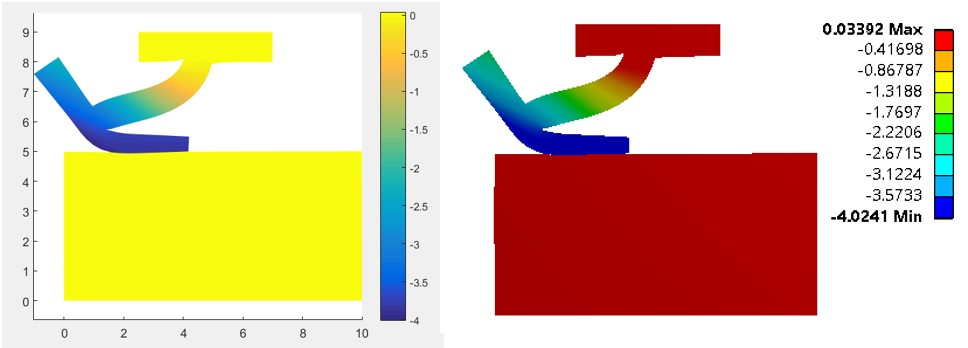
\includegraphics[scale=0.65]{Figures/chapter5/r_q4_ux.jpg}
    \decoRule
    \caption{$u_x$ displacement when using Q4 of rubber example \\
    (MATLAB result in the left, ANSYS result in the right)}
    \label{fig:r_q4_ux}
\end{figure}
\noindent
The $u_x$ displacement of rubber blade example when using 4-nodes element is shown in the Figure \ref{fig:r_q4_ux}.
Maximum volume $u_x$ displacement of MATLAB result is $4.0017 mm$.
Maximum volume $u_x$ displacement of ANSYS result is $4.0241 mm$.
The error of maximum volume $u_x$ displacement between MATLAB result and ANSYS result when using 4-nodes element is $0.55\%$.
So, for maximum volume $u_x$ displacement, the error when using 8-nodes element is lower than when using 4-nodes element.
\newpage
%% COMPARE uy
% uy of q8
\begin{figure}[H]
    \centering
    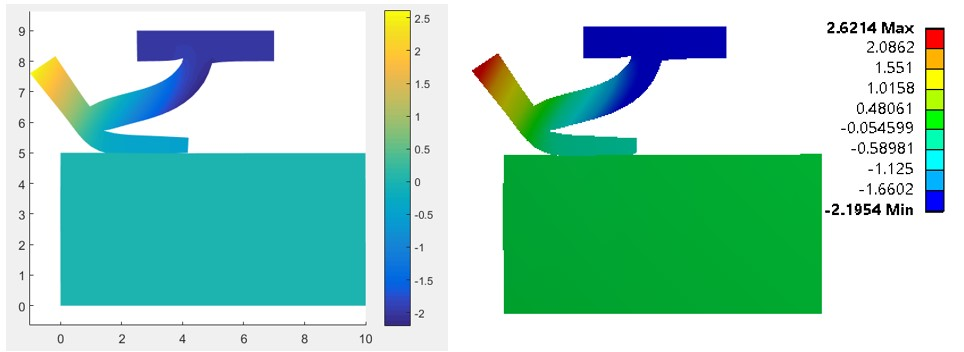
\includegraphics[scale=0.65]{Figures/chapter5/r_q8_uy.jpg}
    \decoRule
    \caption{$u_y$ displacement when using Q8 of rubber example \\
    (MATLAB result in the left, ANSYS result in the right)}
    \label{fig:r_q8_uy}
\end{figure}
\noindent
The $u_y$ displacement of rubber blade example when using 8-nodes element is shown in the Figure \ref{fig:r_q8_uy}.
Maximum volume $u_y$ displacement of MATLAB result is $2.6054 mm$.
Maximum volume $u_y$ displacement of ANSYS result is $2.6214 mm$.
The error of maximum volume $u_y$ displacement between MATLAB result and ANSYS result when using 8-nodes element is $0.61\%$.
\newline
% uy of q4
\begin{figure}[H]
    \centering
    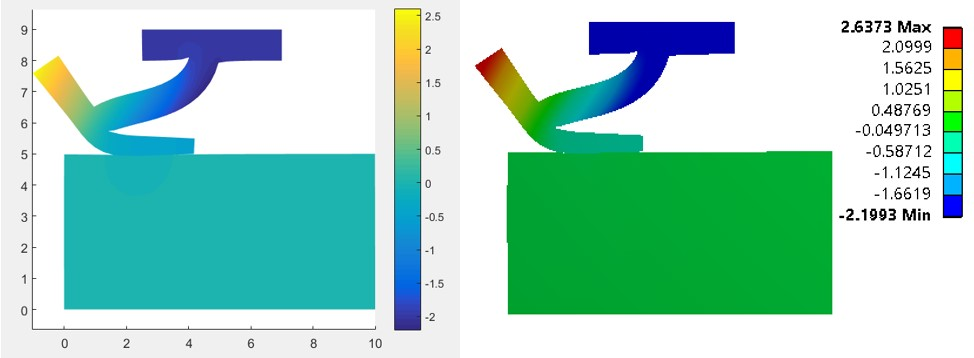
\includegraphics[scale=0.66]{Figures/chapter5/r_q4_uy.jpg}
    \decoRule
    \caption{$u_y$ displacement when using Q4 of rubber example \\
    (MATLAB result in the left, ANSYS result in the right)}
    \label{fig:r_q4_uy}
\end{figure}
\noindent
The $u_y$ displacement of rubber blade example when using 8-nodes element is shown in the Figure \ref{fig:r_q4_uy}.
Maximum volume $u_y$ displacement of MATLAB result is $2.5949 mm$.
Maximum volume $u_y$ displacement of ANSYS result is $2.6373 mm$.
The error of maximum volume $u_y$ displacement between MATLAB result and ANSYS result when using 8-nodes element is $1.61\%$.
So, for maximum volume $u_y$ displacement, the error when using 8-nodes element is lower than when using 4-nodes element.
\vspace{0.38cm}
\newline
Thus, for the rubber blade example, using the 8-nodes element gives more accurate displacement results than using the 4-nodes element.
\newpage
\subsection{Compare stress distribution}
%% COMPARE SX
% sx of q8
\begin{figure}[H]
    \centering
    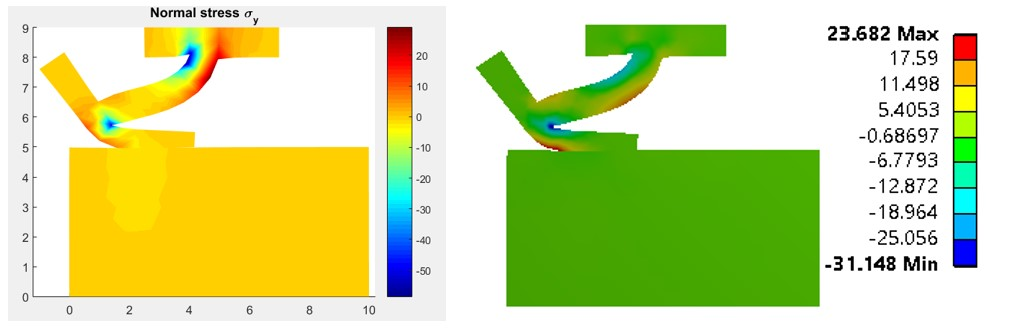
\includegraphics[scale=0.625]{Figures/sx_rub_MvsA.jpg}
    \decoRule
    \caption{Normal stress $\sigma_x$ when using Q8 of rubber example \\
    (MATLAB result in the left, ANSYS result in the right)}
    \label{fig:sx_rub_MandA_5}
\end{figure}
\noindent
The normal stress $\sigma_x$ of rubber blade example when using 8-nodes element is shown in the Figure \ref{fig:sx_rub_MandA_5}.
Maximum normal stress $\sigma_x$ of MATLAB result is $23.4824 MPa$.
Maximum normal stress $\sigma_x$ of ANSYS result is $23.682 MPa$.
The error of maximum normal stress $\sigma_x$ between MATLAB result and ANSYS result when using 8-nodes element is $0.85\%$.
\newline
% sx of q4
\begin{figure}[H]
    \centering
    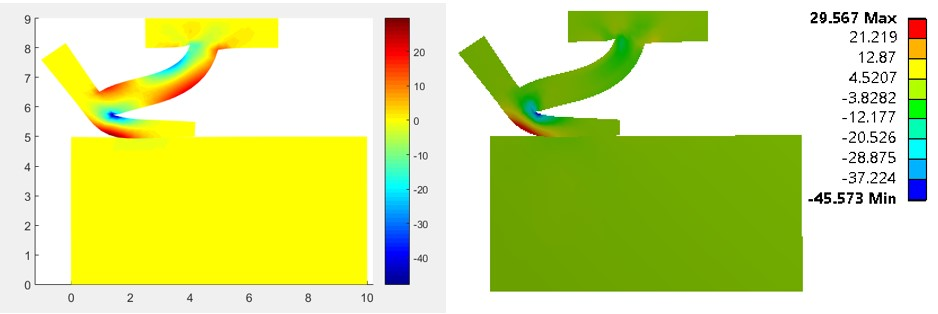
\includegraphics[scale=0.65]{Figures/chapter5/sx_q4_r.jpg}
    \decoRule
    \caption{Normal stress $\sigma_x$ when using Q4 of rubber example \\
    (MATLAB result in the left, ANSYS result in the right)}
    \label{fig:sx_q4_r}
\end{figure}
\noindent
The normal stress $\sigma_x$ of rubber blade example when using 4-nodes element is shown in the Figure \ref{fig:sx_q4_r}.
Maximum normal stress $\sigma_x$ of MATLAB result is $29.6027 MPa$.
Maximum normal stress $\sigma_x$ of ANSYS result is $29.567 MPa$.
The error of maximum normal stress $\sigma_x$ between MATLAB result and ANSYS result when using 8-nodes element is $0.12\%$.
So, for maximum normal stress $\sigma_x$, the error when using 4-nodes element is lower than when using 8-nodes element.
\newpage
%% COMPARE SY
% sx of q8
\begin{figure}[H]
    \centering
    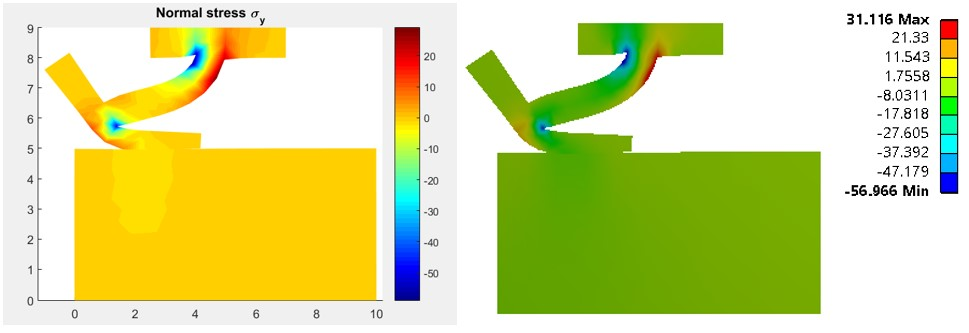
\includegraphics[scale=0.65]{Figures/sy_rub_MvsA.jpg}
    \decoRule
    \caption{Normal stress $\sigma_y$ when using Q8 of rubber example \\
    (MATLAB result in the left, ANSYS result in the right)}
    \label{fig:sy_rub_MandA_5}
\end{figure}
\noindent
The normal stress $\sigma_y$ of rubber blade example when using 8-nodes element is shown in the Figure \ref{fig:sy_rub_MandA_5}.
Maximum normal stress $\sigma_y$ of MATLAB result is $28.9843 MPa$.
Maximum normal stress $\sigma_y$ of ANSYS result is $31.116 MPa$.
The error of maximum normal stress $\sigma_y$ between MATLAB result and ANSYS result when using 8-nodes element is $6.85\%$.
\newline
% sx of q4
\begin{figure}[H]
    \centering
    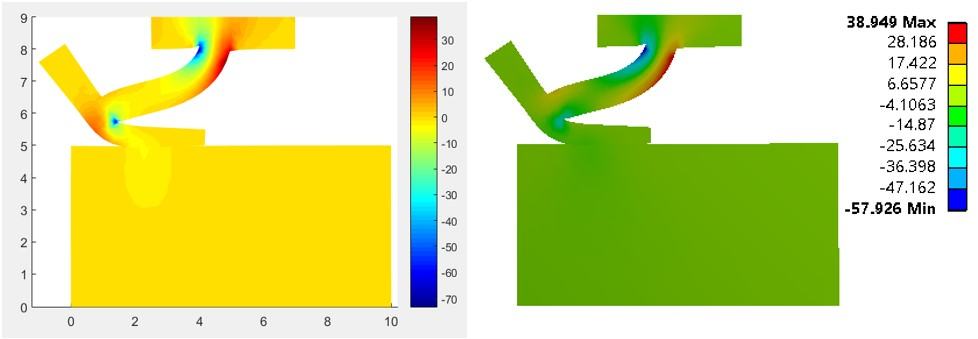
\includegraphics[scale=0.64]{Figures/chapter5/sy_q4_r.jpg}
    \decoRule
    \caption{Normal stress $\sigma_y$ when using Q4 of rubber example \\
    (MATLAB result in the left, ANSYS result in the right)}
    \label{fig:sy_q4_r}
\end{figure}
\noindent
The normal stress $\sigma_y$ of rubber blade example when using 4-nodes element is shown in the Figure \ref{fig:sy_q4_r}.
Maximum normal stress $\sigma_y$ of MATLAB result is $38.6408 MPa$.
Maximum normal stress $\sigma_y$ of ANSYS result is $38.949 MPa$.
The error of maximum normal stress $\sigma_y$ between MATLAB result and ANSYS result when using 8-nodes element is $0.8\%$.
So,  for maximum normal stress $\sigma_y$, the error when using 4-nodes element is lower than when using 8-nodes element.
\vspace{0.38cm}
\newline
Thus, for the rubber blade example, using the 4-nodes element gives more accurate normal stress results than using the 8-nodes element.
\newpage
\section{Synthesis and discussion}
Mesh properties, the soling time and error of displacement and normal stress of self-contact example are shown in Table \ref{tab:sd_s}.
\begin{table}[H]
    \centering
    \begin{tabular}{|l|c|c|}
    \multicolumn{3}{c}{Solution details} \\ \hline
        Details             & 8-nodes element & 4-nodes element  \\ \hline
        Total of node       &{\bf 357 nodes} &445 nodes    \\ \hline
        Total of element    & {\bf 88 elements} &352 elements      \\ \hline
        The solving time    &{\bf 108s}      &       114s      \\ \hline
        Error of maximum volume $u_x$ displacement&{\bf 0.12\%} &0.73\% \\ \hline
        Error of maximum volume $u_y$ displacement&{\bf 0.08\%} &0.10\% \\ \hline
        Error of maximum normal stress $\sigma_x$ &{\bf 1.13\%}&7\% \\ \hline
        Error of maximum normal stress $\sigma_y$ &{\bf 0.18\%}&5.7\% \\ \hline
    \end{tabular}
    \caption{Solution details of self-contact example}
    \label{tab:sd_s}
\end{table}
\noindent
Mesh properties, the soling time and error of displacement and normal stress of rubber blade example are shown in Table \ref{tab:sd_r}.
\begin{table}[H]
    \centering
    \begin{tabular}{|l|c|c|}
    \multicolumn{3}{c}{Solution details} \\ \hline
        Details             & 8-nodes element & 4-nodes element  \\ \hline
        Total of node       &{\bf 435 nodes} &548 nodes    \\ \hline
        Total of element    & {\bf 113 elements} &452 elements      \\ \hline
        The solving time    &{\bf 75s}      &       79s      \\ \hline
        Error of maximum volume $u_x$ displacement&{\bf 0.21\%} &0.55\% \\ \hline
        Error of maximum volume $u_y$ displacement&{\bf 0.61\%} &1.61\% \\ \hline
        Error of maximum normal stress $\sigma_x$ &0.85\%&{\bf 0.12\%} \\ \hline
        Error of maximum normal stress $\sigma_y$ & 6.85\%&{\bf 0.8\%} \\ \hline
    \end{tabular}
    \caption{Solution details of rubber blade example}
    \label{tab:sd_r}
\end{table}
\noindent
From the two examples, we can see that with the above meshing method, the 8-node element has a faster computation time and a more accurate displacement result.
That's probably because the quadratic approximation of the 8-nodes element (keeping the same size) leads to the small error for the solution.
\vspace{0.38cm}
\newline
From the two examples, we cannot confirm that using the 8-node element together with reducing the number of elements by four times gives a more accurate result than the 4-node element.
Although the quadratic approximation helps to reduce the error, too much reduction in the number of elements also adversely affects the result.
\vspace{0.01cm}
\newline
The comparison of the 8-nodes and the 4-nodes also shows that the 8-nodes are effective in meshing on the curve.
